\documentclass[11pt,a4paper]{article}
\usepackage[margin=2.3cm]{geometry}
\usepackage[T1]{fontenc}
\usepackage{textcomp}
\input{glyphtounicode}
\pdfgentounicode=1
\usepackage{lmodern}
\usepackage{amsmath}
\usepackage{xcolor}
\usepackage{listings}
\usepackage{tcolorbox}
\tcbuselibrary{breakable}
\usepackage{booktabs}
\usepackage{array}
\usepackage{tikz}
\usepackage{float}
\usepackage{graphicx}
\graphicspath{{images/}}
\usepackage{hyperref}
\hypersetup{colorlinks=true, linkcolor=blue!50!black, citecolor=green!40!black}

\usepackage{accsupp}
% line numbers are drawn but excluded from copied text
\newcommand{\nocopy}[1]{\BeginAccSupp{method=escape,ActualText={}}#1\EndAccSupp{}}
\lstset{
  language=C, basicstyle=\ttfamily\small, keywordstyle={}, commentstyle={}, stringstyle={},
  numbers=left, numberstyle=\footnotesize\nocopy, numbersep=10pt, xleftmargin=2.4em,
  frame=none, columns=fullflexible, keepspaces=true, upquote=true, showstringspaces=false,
  breaklines=true, captionpos=b, aboveskip=1em, belowskip=0.8em
}
\lstdefinestyle{sh}{language=bash, numbers=none, xleftmargin=2.4em}
\renewcommand{\lstlistingname}{Listing}
% code names in the text: grey monospace
\let\origtexttt\texttt
\renewcommand{\texttt}[1]{\textcolor{black!60}{\origtexttt{#1}}}

\newtcolorbox{keyidea}{colback=blue!4, colframe=blue!45!black, title=Key ideas, fonttitle=\bfseries\small}
\newtcolorbox{experiment}{breakable, colback=orange!5, colframe=orange!70!black, title=Experiment, fonttitle=\bfseries\small}

\title{\textbf{OpenMP Tasks: Dependencies with \texttt{depend}}\\[4pt]\large Lesson 13: ordering tasks by the data they read and write}
\author{Gustavo Lozano}
\date{November 2026}

\begin{document}
\maketitle

\noindent\textit{\small Source: van der Pas, Stotzer \& Terboven~\cite{vdp}, chapter on tasking
(task dependences, added in OpenMP~4.0). Prerequisite: \texttt{00-openmp\_tasks.pdf} (Lesson 12).}

\section{The idea}
In Lesson~12 the only way to wait for tasks was \texttt{taskwait}: wait for \emph{all} the
children. Often that is far too strong. Here, each of $8$ blocks goes through two stages:
stage~1 writes \texttt{x[b]}, stage~2 reads \texttt{x[b]} and writes \texttt{y[b]}. Stage~2 of
block $b$ only needs stage~1 of the \emph{same} block.

\begin{figure}[H]
\centering
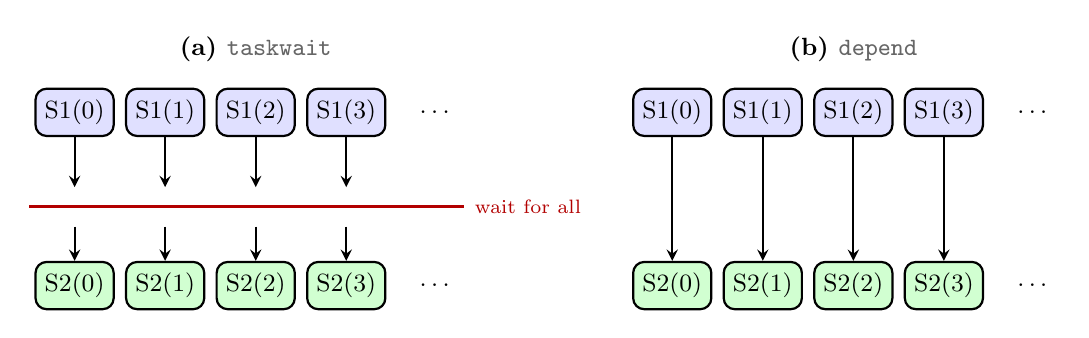
\begin{tikzpicture}[thick, font=\small, x=1.15cm, y=1cm,
  s1/.style={draw, rounded corners, fill=blue!12, minimum width=0.95cm, minimum height=0.6cm},
  s2/.style={draw, rounded corners, fill=green!18, minimum width=0.95cm, minimum height=0.6cm},
  bar/.style={draw=red!70!black, very thick}]
  
  \node[font=\small\bfseries] at (2,1.1) {(a) \texttt{taskwait}};
  \foreach \b in {0,...,3} {
    \node[s1] (a\b) at (\b,0.3) {S1(\b)};
    \node[s2] (c\b) at (\b,-1.9) {S2(\b)};
    \draw[->,>=stealth] (a\b) -- (\b,-0.65);
    \draw[->,>=stealth] (\b,-1.15) -- (c\b);
  }
  \node at (4,0.3) {\ldots}; \node at (4,-1.9) {\ldots};
  \draw[bar] (-0.5,-0.9) -- (4.3,-0.9) node[right, font=\scriptsize, text=red!70!black] {wait for all};
  
  \node[font=\small\bfseries] at (8.6,1.1) {(b) \texttt{depend}};
  \foreach \b in {0,...,3} {
    \node[s1] (d\b) at (6.6+\b,0.3) {S1(\b)};
    \node[s2] (e\b) at (6.6+\b,-1.9) {S2(\b)};
    \draw[->,>=stealth] (d\b) -- (e\b);
  }
  \node at (10.6,0.3) {\ldots}; \node at (10.6,-1.9) {\ldots};
\end{tikzpicture}
\caption{(a) With \texttt{taskwait}, every S2 waits for every S1. (b) With \texttt{depend},
S2($b$) waits only for S1($b$).}
\end{figure}

\section{The \texttt{depend} clause}
A task declares which data it reads (\texttt{in}) and writes (\texttt{out}). OpenMP starts a
task only when the earlier tasks it conflicts with have finished:
\begin{center}
\small
\begin{tabular}{@{}lll@{}}
\toprule
Earlier task & Later task & Later task waits? \\ \midrule
\texttt{out: x[b]} & \texttt{in: x[b]}  & yes (read after write) \\
\texttt{in: x[b]}  & \texttt{out: x[b]} & yes (write after read) \\
\texttt{out: x[b]} & \texttt{out: x[b]} & yes (write after write) \\
\texttt{in: x[b]}  & \texttt{in: x[b]}  & no: two readers can run together \\
\bottomrule
\end{tabular}
\end{center}
``Earlier'' means created earlier by the same parent, so the order in which tasks are
\emph{created} defines the order of the dependent ones. Tasks without a conflict run as soon
as a thread is free.

\begin{lstlisting}
#pragma omp task depend(out: x[b])                  /* S1: writes x[b] */
stage1(b);
#pragma omp task depend(in: x[b]) depend(out: y[b]) /* S2: waits for S1(b) only */
stage2(b);
\end{lstlisting}

\section{The code}
Stage costs are chosen so that the difference shows: block 0 is slow in stage~1 (100\,ms,
the others 10\,ms); in stage~2 it is the other way round (block 0: 10\,ms, the others
100\,ms). The work is simulated with \texttt{usleep}, so the times do not depend on your CPU.
Each stage records the thread that ran it and its start and end times (ms since the start of
the version); \texttt{report} prints them as a table.

\lstinputlisting[caption={\textbf{\origtexttt{depend\_pipeline.c}} -- two-stage pipeline, with \origtexttt{taskwait} and with \origtexttt{depend}.}, label={lst:dep}]{depend_pipeline.c}

\begin{lstlisting}[style=sh]
gcc -Wall -O2 -fopenmp -o depend_pipeline depend_pipeline.c
OMP_NUM_THREADS=8 ./depend_pipeline
\end{lstlisting}

\begin{figure}[H]
\centering
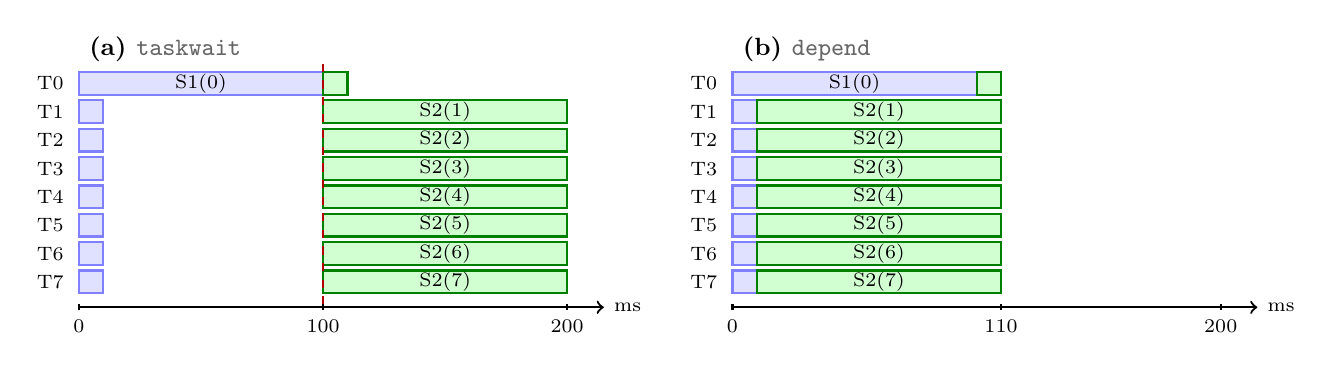
\begin{tikzpicture}[thick, font=\scriptsize, x=0.031cm, y=0.36cm,
  s1/.style={draw=blue!50, fill=blue!12}, s2/.style={draw=green!50!black, fill=green!18}]
  \node[font=\small\bfseries, anchor=west] at (0,9.6) {(a) \texttt{taskwait}};
  \foreach \t in {0,...,7} \node[anchor=east] at (-2,8-\t+0.4) {T\t};
  \draw[s1] (0,8) rectangle (100,8.8); \node at (50,8.4) {S1(0)};
  \draw[s2] (100,8) rectangle (110,8.8);
  \foreach \t in {1,...,7} {
    \draw[s1] (0,8-\t) rectangle (10,8.8-\t);
    \draw[s2] (100,8-\t) rectangle (200,8.8-\t); \node at (150,8.4-\t) {S2(\t)};
  }
  \draw[red!70!black, dashed] (100,0.6) -- (100,9.2);
  \draw[->] (0,0.5) -- (215,0.5) node[right] {ms};
  \foreach \x in {0,100,200} {\draw (\x,0.4) -- (\x,0.6); \node[below] at (\x,0.4) {\x};}
  
  \begin{scope}[xshift=8.3cm]
  \node[font=\small\bfseries, anchor=west] at (0,9.6) {(b) \texttt{depend}};
  \foreach \t in {0,...,7} \node[anchor=east] at (-2,8-\t+0.4) {T\t};
  \draw[s1] (0,8) rectangle (100,8.8); \node at (50,8.4) {S1(0)};
  \draw[s2] (100,8) rectangle (110,8.8);
  \foreach \t in {1,...,7} {
    \draw[s1] (0,8-\t) rectangle (10,8.8-\t);
    \draw[s2] (10,8-\t) rectangle (110,8.8-\t); \node at (60,8.4-\t) {S2(\t)};
  }
  \draw[->] (0,0.5) -- (215,0.5) node[right] {ms};
  \foreach \x in {0,110,200} {\draw (\x,0.4) -- (\x,0.6); \node[below] at (\x,0.4) {\x};}
  \end{scope}
\end{tikzpicture}
\caption{8 threads, one possible assignment of tasks to threads. (a) The stage-2 tasks wait
90\,ms for S1(0): 200\,ms in total. (b) Each S2($b$) starts right after its own S1($b$):
110\,ms.}
\end{figure}
Output with 8 threads (the thread numbers change from run to run):
\begin{lstlisting}[style=sh, basicstyle=\ttfamily\footnotesize]
barrier : 0.201 s   correct: yes
  block | stage1: thread start  end | stage2: thread start  end   (ms)
      0 |             2     0  101 |             4   101  111
      1 |             0     0   10 |             3   101  201
      2 |             1     0   11 |             5   101  201
      3 |             4     0   11 |             6   101  201
      4 |             5     0   10 |             7   101  201
      5 |             6     0   10 |             1   101  201
      6 |             3     0   10 |             0   101  201
      7 |             7     0   10 |             2   101  201
depend  : 0.111 s   correct: yes
  block | stage1: thread start  end | stage2: thread start  end   (ms)
      0 |             4     0  100 |             4   100  110
      1 |             1     0   10 |             1    10  110
      2 |             0     0   10 |             0    10  110
      3 |             2     0   10 |             2    10  110
      4 |             7     0   10 |             7    10  110
      5 |             3     0   10 |             3    10  110
      6 |             6     0   10 |             6    10  110
      7 |             5     0   10 |             5    10  111
threads = 8
\end{lstlisting}
In the \texttt{barrier} table every stage~2 starts at about 101\,ms, after S1(0) ends; in the
\texttt{depend} table S2($b$) starts when S1($b$) ends (10\,ms, or 100\,ms for block 0).
S1(0) ran on thread 2 in the first version and on thread 4 in the second: any thread can run any task.

\begin{keyidea}
\begin{itemize}
  \item \texttt{depend} replaces ``wait for everything'' by ``wait for what I read'': a task
        waits only for the earlier tasks that write the data it uses.
  \item Dependencies are declared on data (\texttt{x[b]}), not on tasks; the order of task
        creation decides which task is ``earlier''.
  \item Independent work keeps flowing, so the idle time at barriers disappears.
\end{itemize}
\end{keyidea}

\section{The experiment}
\begin{experiment}
\textbf{Question:} when does \texttt{depend} pay off, and what happens if a dependency is
missing?
\begin{enumerate}
  \item Run with several thread counts:
\begin{lstlisting}[style=sh]
for t in 1 2 4 8; do OMP_NUM_THREADS=$t ./depend_pipeline; echo; done
\end{lstlisting}
  \item Remove \texttt{depend(in: x[b])} from the stage-2 task (line~96 of
        Listing~\ref{lst:dep}), recompile, and run three times with 4 threads.
\end{enumerate}
\textbf{What to observe and answer.}
\begin{enumerate}
  \item With 1 thread both versions take the same time. Why?
  \item With 8 threads, explain the two times (about 0.20\,s and 0.11\,s) from the costs of
        the stages.
  \item Without \texttt{depend(in: x[b])} the program is faster but prints
        \texttt{correct: NO}. What went wrong?
\end{enumerate}
\end{experiment}

\paragraph{Answers (read after trying).}

\noindent(1)~One thread runs every task one after another: $100 + 7\cdot10 + 10 + 7\cdot100 =
880$\,ms in both versions. Dependencies only change \emph{when} tasks may start, and with one
thread there is nothing to overlap.

\noindent(2)~With \texttt{taskwait}, no stage-2 task can start before S1(0) ends at 100\,ms;
then S2(1)--S2(7) take 100\,ms more: 200\,ms. With \texttt{depend}, S2($b$) starts right after
S1($b$) at 10\,ms and ends at 110\,ms, while S1(0) and S2(0) end at 110\,ms too: 110\,ms
(Figure~2).

\noindent(3)~Without the \texttt{in} dependency, stage~2 of a block may run before stage~1 of the
same block has written \texttt{x[b]}; it then reads the old value 0 and writes
$\texttt{y[b]} = 0$. It is faster only because it waits for nothing. A missing dependency is
a data race, like the ones in Lessons~2 and 10.

\paragraph{Second example.} A realistic use of \texttt{depend}: the sparse triangular solve
from Saad~\cite{saad}, in\\ \texttt{01-openmp\_task\_depend\_trsv.pdf}.

\begin{thebibliography}{9}
\bibitem{vdp} R.~van der Pas, E.~Stotzer, and C.~Terboven. \emph{Using OpenMP --- The Next
  Step: Affinity, Accelerators, Tasking, and SIMD}. MIT Press, Cambridge, MA, 2017.
\bibitem{saad} Y.~Saad. \emph{Iterative Methods for Sparse Linear Systems}, 2nd ed. SIAM,
  Philadelphia, PA, 2003.
\end{thebibliography}
\end{document}
